\documentclass{article}
\usepackage[en]{ukon-infie}
\usepackage[utf8]{inputenc}
\usepackage{algorithm2e}
\usepackage{amsmath}
\usepackage{graphicx}
\usepackage{hyperref}
% kann de oder en sein
% kann bubble break, topexercise sein

\Names{Jonas Probst, Simon Giebenhain}
\Lecture[AnaVis]{Analyse und Visualisierung von Informationen}
\Term{WS 2017/18}

\begin{document}
    \begin{ukon-infie}[31.01.18]{11}

        \begin{exercise}[p=3]{Temporal Data}  
        \question{}
        {
        Whereas static temporal data is a view of historic observations and therefore does not change anymore, dynamic temporal data is data which is periodically updated.
      	}
      	
      	\question{}
      	{
      	Whereas linear temporal data assumes a starting point and tracks data until the present/future or some ending point, cyclic temporal data stores observations in recurrent time intervals/points.
      	}
      	\question{}
      	{
      	Time points have no duration (like a snapshot of that moment), where as time intervals are defined by a start and an ending point.
      	}
		\end{exercise}
		
		
		\begin{exercise}[p=7]{Choose a Visualization for Temporal Data}
		\question{}
		{
		The data is static, since it contains data of the past, that is, the data is not updated anymore.\\
		Futhermore it is linear, because the data starts from he 12th of August and ends at some unknown day, collecting data for every day inbetween.\\
		Open and close(value of first/last transaction per day) are time point data and High,Low and Volume are time interval data, because they take the whole day into account.
		}
		\question{}
		{
		
		\textbf{Note:} It does not make sense to compare the values of a single share, because that heavily depends on the total number of shares available. The market capitalization would make more sense (multiply current price with number of shares).\\
		
			We chose the \textbf{TimeSearcher} visualization method, which displays the stocks by multiple line-plots. To improve visibility one would somehow compute an average price for each day and from this compute the market capitalization, if possible. Thereby we lose some details, but this is necessary to maintain visibility.\\
			
						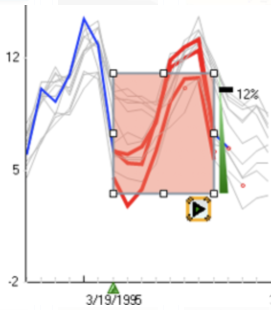
\includegraphics[scale=0.7]{time_searcher.png}
						
						As can be seen in the picture, the user can select a subset of the plots he/she wants to investigate. This increases the effectiveness of the visualization, by reducing the choas inflicted by the large number of stocks. Furthermore the timebox query enables the user to zoom in on areas(time intervals) of interest. This is especially useful to e.g. investigate the effect of certain historic events on the stocks.\\

			
			However one could think about replacing the line-plot with a candle-scatter-plot, as can be seen below. The advantage of the candles is that it expresses open, close, high and low in one symbol. Additionally the volume can be displayed below, as a stacked bar chart, because it does not fit in the same grpah has the outher attributes. Then we might have a problem with overplotting, though.
			
						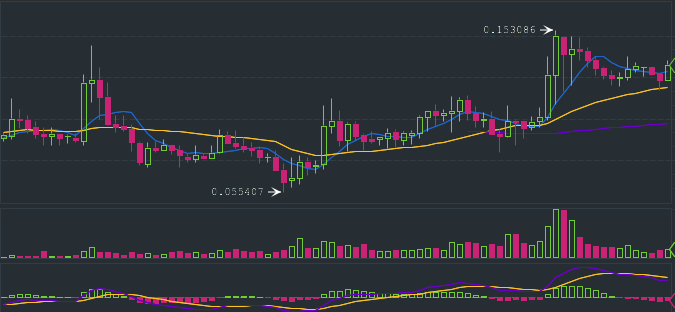
\includegraphics[scale=0.7]{candles.png}

			\tiny source: \url{https://www.binance.com/tradeDetail.html?symbol=NEO_ETH}
			\normalsize \\
			
			Another approach to visualize temporal data is with a layer area graph:\\
			
			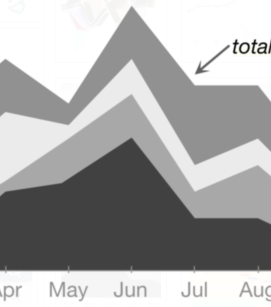
\includegraphics[scale=0.7]{layered_area_graph.png}
			
			This can be very misleading in our example, because one might think that a stock is rising, whereas this is only caused, by a the changes in other stocks. Furthermore one might value the stocks on top of layered graph higher than the lower ones. It takes much more attention to actually understand what is going on. Also it would be hard to incorporate more than on of the variables open, close, high,low, volume in a single graph.
			
			
		}
		\end{exercise}
		
		\begin{exercise}[p=4]{Pixel-oriented Visualization}
		
		\end{exercise}
		
		
\end{ukon-infie}
\end{document}
